\documentclass{beamer}
\mode<presentation>
\usetheme{CambridgeUS}
\usepackage[russian]{babel}
\usepackage[utf8]{inputenc}
\usepackage[T2A]{fontenc}
\usepackage{sansmathaccent}
\pdfmapfile{+sansmathaccent.map}
\title{Динамическая обработка сигналов}
\author{Наумов Д.А.}
\date[01.04.2014] {Компьютерные музыкальные технологии и звуковой дизайн, 2014}

\begin{document}

%ТИТУЛЬНЫЙ СЛАЙД
\begin{frame}
  \titlepage
\end{frame}

%СОДЕРЖАНИЕ ЛЕКЦИИ
\begin{frame}
  \frametitle{Содержание лекции}
  \tableofcontents
\end{frame}

%РАЗДЕЛ 1
\section{Основные понятия}
\begin{frame}
\textbf{Динамическая обработка звука}~--- обработка, которая приводит к изменению динамического диапазона фонограммы.

~

Под \textbf{динамическим диапазоном сигнала} понимают отношение максимального и минимального уровней громкости (\emph{maximum}, \emph{minimum RMS power}).

~

Из всех процессов, используемых в создании музыки, динамическая обработка звука является, пожалуй, наиболее сложной для восприятия. В первую очередь это связано с тем, что зачастую результат обработки звука едва различим на слух~--- особенно для начинающих. Другая трудность заключается в количестве изменяемых параметров: их не так мало, и к тому же, изменение каждого из них не всегда приводит к очевидным результатам.
\end{frame}

\begin{frame}
  \begin{block}{Сигналограмма фрагмента оперы С. Рахманинова "<Алеко">}
    \centering{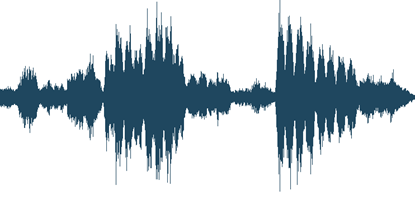
\includegraphics[width=0.5\textwidth]{pic-signal-01}}
  \end{block}
  \begin{block}{Сигналограмма современной танцевальной музыки}
    \centering{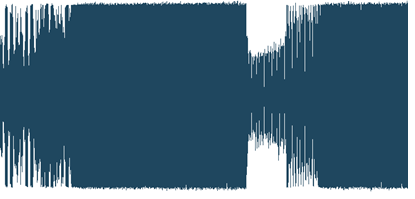
\includegraphics[width=0.5\textwidth]{pic-signal-02}}
  \end{block}
\end{frame}

\begin{frame}
  \begin{block}{Задачи, решаемые при помощи динамической обработке}
    \begin{itemize}
       \item выравнивание динамики звука (например, речи);
       \item увеличение громкости звучания без изменения пиковой амплитуды (например, звука большого барабана);
       \item уменьшение громкости отдельных составляющих (например, шипящих звуков);
       \item подавление фонового шума, отличающегося по уровню от полезного сигнала;
       \item ограничение уровня сигнала (например, для того, чтобы избежать клипирования).
    \end{itemize}
  \end{block}
\end{frame}

\begin{frame}
  Любой инструмент динамической обработки имеет три функциональных элемента:
  \begin{itemize}
    \item основной канал;
    \item детектор огибающей;
    \item контроллер громкости.
  \end{itemize}

  ~

  Задачи \textbf{детектора огибающей}~--- обнаружить момент пересечения аудио сигналом из основного канала порогового значения и измерить уровень аудио сигнала   относительно данного по-рогового значения.

  ~

  Задача \textbf{контроллера громкости}~--- выработать управляющее воздействие на основной канал в зависимости от измеренной величины аудио сигнала.
\end{frame}

\begin{frame}
  В зависимости от параметров контроллера громкости и детектора огибающей, различают следующие инструменты динамической обработки:
  \begin{itemize}
    \item компрессор (\textit{compressor});
    \item экспандер (\textit{expander});
    \item лимитер (\textit{limiter});
    \item автостабилизатор (\textit{auto stabilizer});
    \item шумоподавитель (\textit{noise gate});
    \item устройства со сложным преобразованием динамического диапазона.
  \end{itemize}
\end{frame}

\section{Компрессор}
\begin{frame}
  \textbf{Компрессор}~--- это инструмент динамической обработки, который уменьшает динамический диапазон сигнала и, благодаря этому, уменьшает разницу в уровне  громкости между тихими и громкими звуками.

  \begin{block}{Сигналограмма исходного сигнала}
    \centering{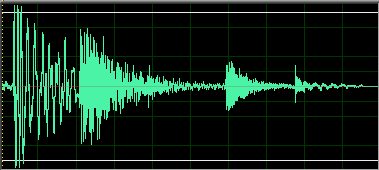
\includegraphics[width=0.4\textwidth]{pic-example-01}}
  \end{block}

  \begin{block}{Сигналограмма сигнала после обработки компрессором}
    \centering{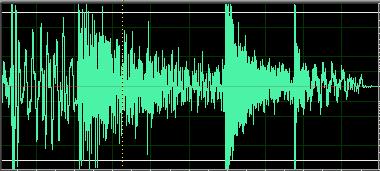
\includegraphics[width=0.4\textwidth]{pic-example-02}}
  \end{block}
\end{frame}

\begin{frame}
  Результат динамической обработки зависит от правильного выбора значений нескольких основных параметров. К важнейшим из них относятся:
  \begin{itemize}
    \item порог срабатывания (\emph{threshold});
    \item коэффициент компрессии (\emph{ratio});
    \item компенсирующее усиление (\emph{makeup gain});
    \item время атаки (\emph{attack time});
    \item время восстановления (\emph{release time}).
  \end{itemize}

  ~

  \textbf{Порог срабатывания} задает уровень громкости, при превышении которого начинается управление усилением. До тех пор, пока значение уровня сигнала меньше порогового, обработка не воздействует на сигнал.
\end{frame}

\begin{frame}
  \begin{block}{Сигналограмма исходного сигнала}
    \centering{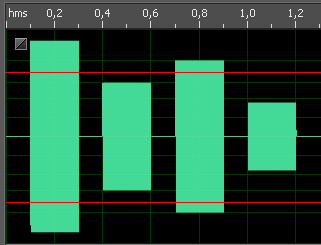
\includegraphics[width=0.35\textwidth]{pic-compress-01}}
  \end{block}

  \begin{block}{Сигналограмма сигнала после обработки компрессором}
    \centering{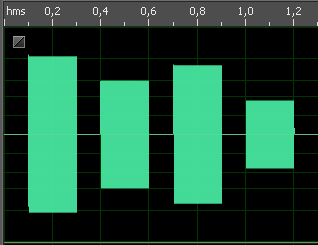
\includegraphics[width=0.35\textwidth]{pic-compress-02}}
  \end{block}
\end{frame}

\begin{frame}
  \textbf{Коэффициент компрессии} определяет степень сжатия динамического диапазона сигнала, имеющего уровень выше порогового.

  \begin{block}{Сигналограммы сигналов после обработки компрессором с коэффициентами 1:1, 2:1, 4:1, 8:1}
    \centering{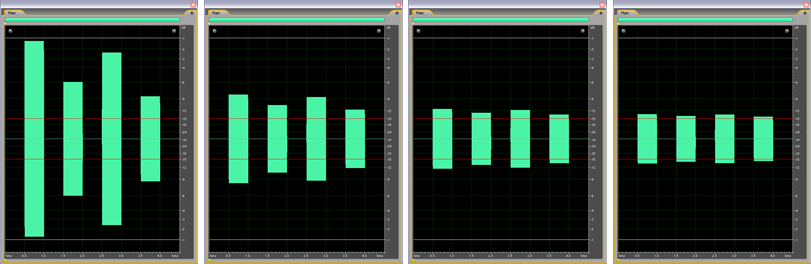
\includegraphics[width=0.85\textwidth]{pic-compress-07}}
  \end{block}
\end{frame}

\begin{frame}
  \textbf{Компенсирующее усиление} необходимо для того, чтобы усилить сигнал, который был ослаблен при выполнении динамической обработки.

  \begin{block}{Компрессия с коэффициентами 2:1, 4:1, 8:1}
     \centering{ 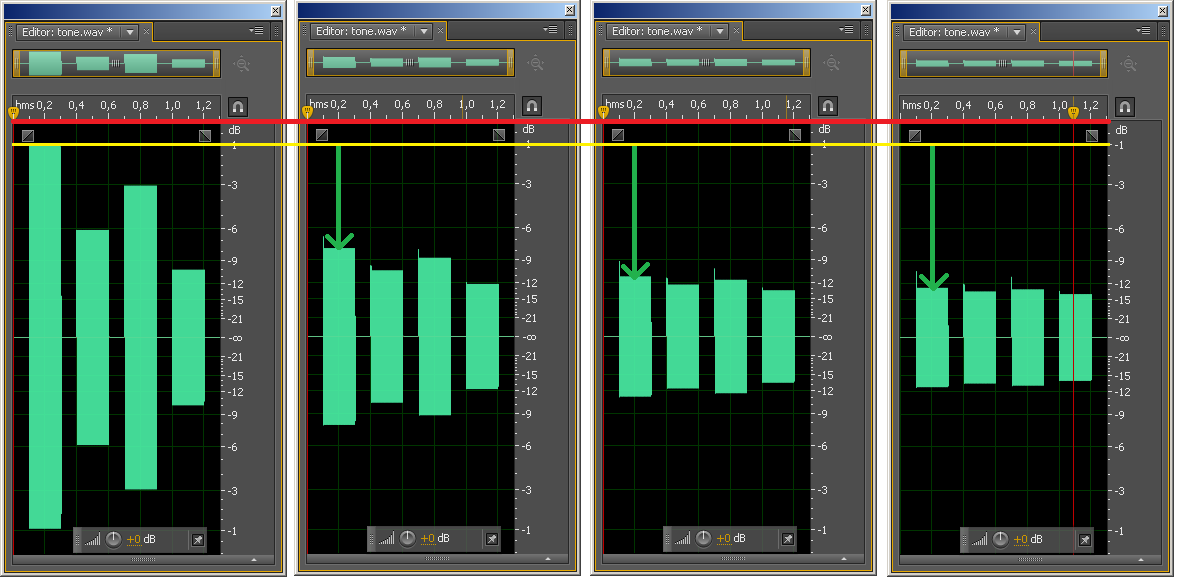
\includegraphics[width=0.95\textwidth]{pic-compress-03}}
  \end{block}
\end{frame}

\begin{frame}
  Оценку инерционности устройств динамической обработки осуществляют на основе анализа двух временных характеристик:
  \begin{itemize}
    \item \textbf{время атаки} (\emph{attack time})~--- время реакция устройства на увеличение уровня сигнала;
    \item \textbf{время восстановления }(\emph{release time})~--- время реакция устройства на уменьшение уровня сигнала.
  \end{itemize}

  \begin{block}{Влияние времени атаки на форму сигнала}
    \centering{ 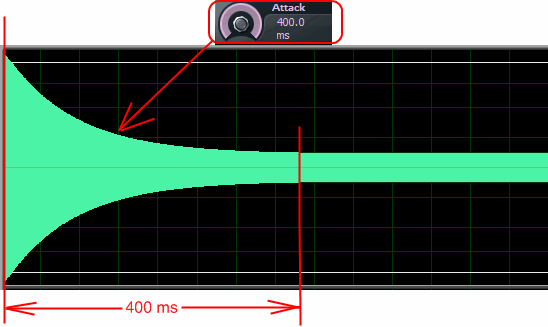
\includegraphics[width=0.75\textwidth]{pic-compress-04}}
  \end{block}
\end{frame}

\begin{frame}
  \begin{block}{Пример компрессии со временем атаки 0.05, 1 и 100 мсек}
    \centering{ 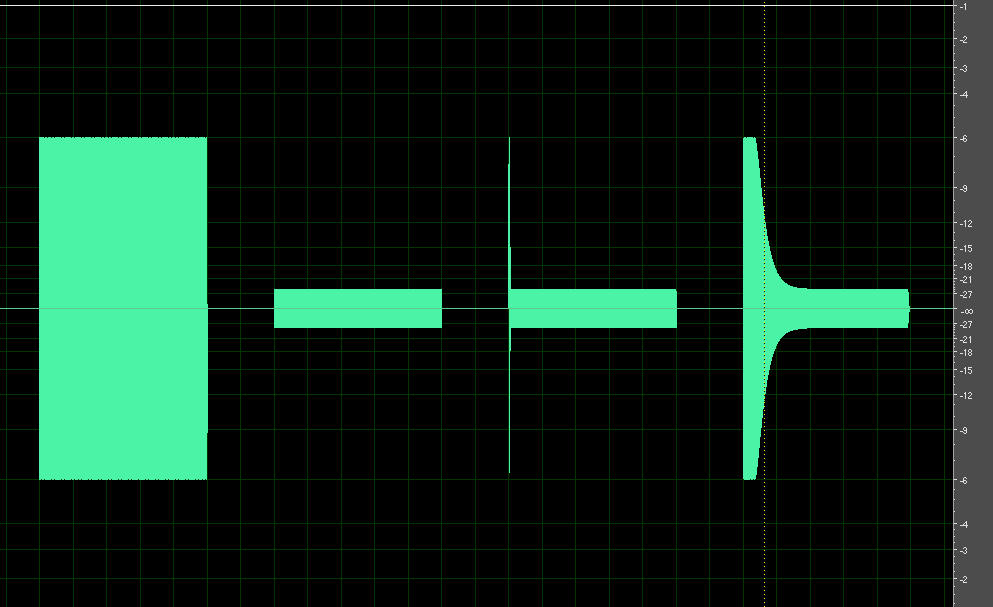
\includegraphics[width=0.75\textwidth]{pic-compress-05}}
  \end{block}
\end{frame}

\begin{frame}
  \textbf{Время восстановления}~--- время, за которое устройство динамической обработки выходит из активного состояния после падения уровня сигнала ниже порогового.

  \begin{block}{Влияние времени восстановления на форму сигнала}
    \centering{ 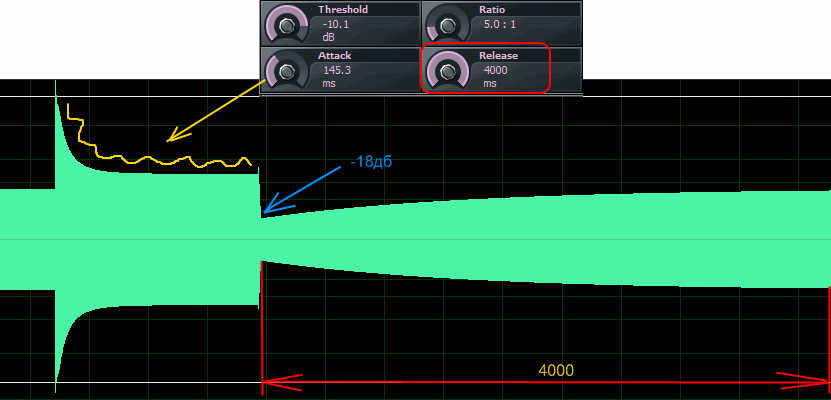
\includegraphics[width=0.75\textwidth]{pic-compress-06}}
  \end{block}
\end{frame}

\begin{frame}
  \textbf{Амплитудная характеристика}~--- график зависимости уровня выходного сигнала от уровня выходного сигнала.

  \begin{block}{Амплитудная характеристика компрессора}
    \centering{ 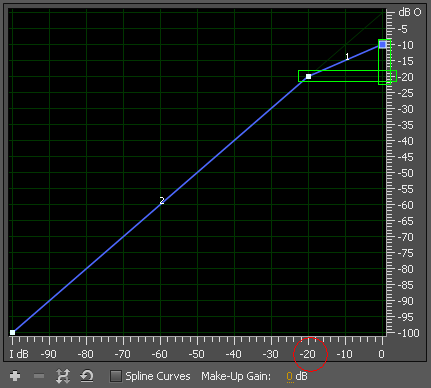
\includegraphics[width=0.6\textwidth]{pic-amp-01}}
  \end{block}
\end{frame}

\begin{frame}
  \begin{block}{Амплитудная характеристика сложного инструмента динамической обработки}
    \centering{ 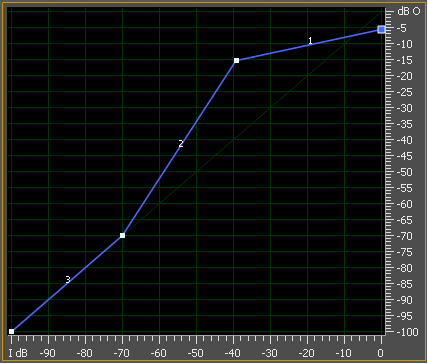
\includegraphics[width=0.6\textwidth]{pic-amp-02}}
  \end{block}
\end{frame}

\section{Экспандер, лимитер, гейт}
\begin{frame}
  \textbf{Экспандер} динамического диапазона применяют в том случае, когда необходимо расширить динамический диапазон сигнала.

  \begin{block}{Амплитудная характеристика экспандера}
    \centering{ 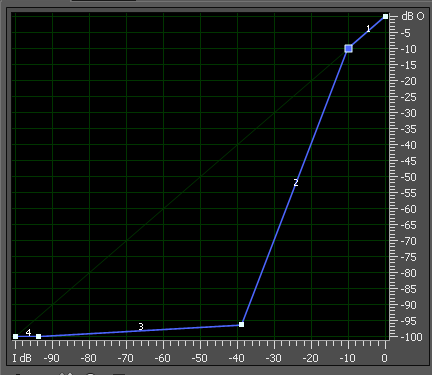
\includegraphics[width=0.6\textwidth]{pic-exp-01}}
  \end{block}
\end{frame}

\begin{frame}
  \textbf{Пороговый шумоподавитель} (\emph{гейт}, \emph{noise gate}, \emph{gate})~--- предназначен для подавления сигнала, который находится в заданном динамическом диапазоне.

  \begin{block}{Амплитудная характеристика однопорогового гейта}
    \centering{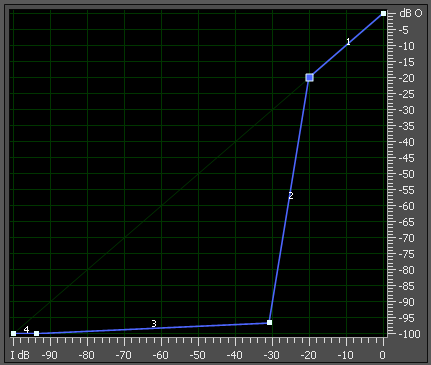
\includegraphics[width=0.6\textwidth]{pic-gate-01}}
  \end{block}
\end{frame}

\begin{frame}
  \begin{block}{Амплитудная характеристика однопорогового гейта}
    \centering{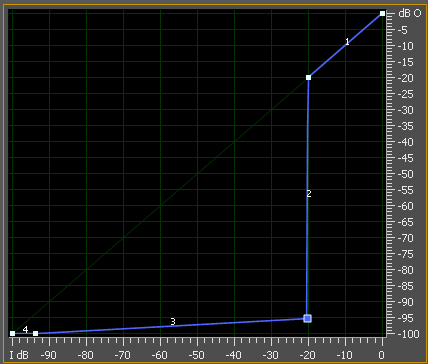
\includegraphics[width=0.6\textwidth]{pic-gate-02}}
  \end{block}
\end{frame}

\begin{frame}
  \textbf{Лимитер} (\emph{limiter}, ограничитель уровня)~--- ограничитель динамического диапазона, в большинстве случаев используется для предотвращения перегрузки (клипирования) и подавления кратковременных всплесков громкости (пиков), при выравнивании динамики сигнала. В последовательности эффектов лимитер обычно стоит последним.

  \begin{block} {Амплитудная характеристика лимитера}
    \centering{ 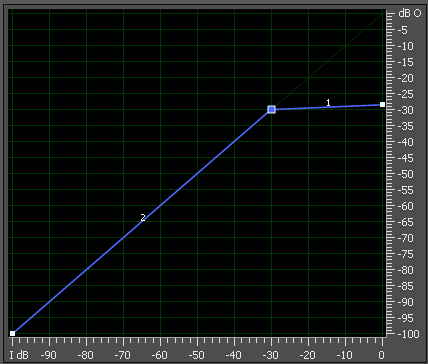
\includegraphics[width=0.5\textwidth]{pic-limiter-01}}
  \end{block}
\end{frame}

\section[Adobe Audition]{Инструменты динамической обработки Adobe Audition}
\begin{frame}
  В составе \emph{Adobe Audition} имеются следующие инструменты динамической обработки:
  \begin{itemize}
    \item \emph{Dynamics Processing}~--- универсальная динамическая обработка;
    \item \emph{Hard Limiting}~--- ограничитель уровня;
    \item \emph{Single-band compressor}~--- однополосный компрессор;
    \item \emph{Tube-modeled compressor}~--- инструмент, эмулирующий старые аппаратные устройства-компрессоры;
    \item \emph{Multiband compressor}~--- многополосный компрессор.
  \end{itemize}
\end{frame}

\begin{frame}
  Диалоговое окно \emph{Dynamics Processing} открывается командой \emph{Effects > Amplitude And Compression > Dynamics Processing}. В зависимости от выбранных значений параметров данный эффект может выполнять функции гейта, компрессора, экспандера, лимитера и т.д.

  \begin{block} {Окно инструмента \emph{Dynamics Processing}}
    \centering{ 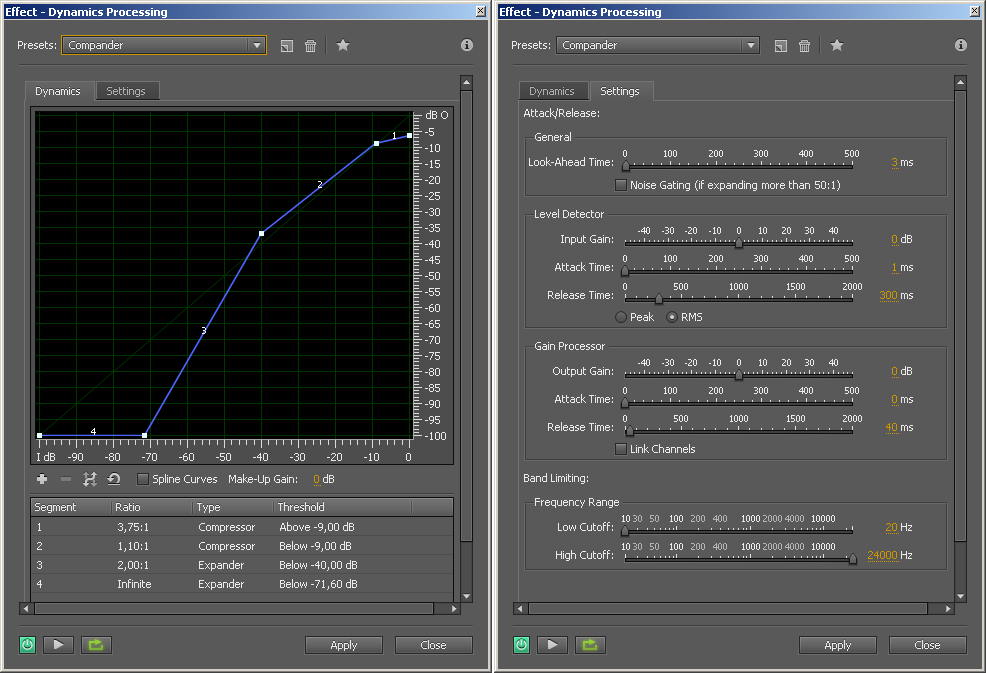
\includegraphics[width=0.5\textwidth]{pic-dynamic-01}}
  \end{block}
\end{frame}

\begin{frame}
  Команда \emph{Effects > Amplitude and Compression > Hard Limiting} открывает диалоговое окно \emph{Hard Limiting}.

  \begin{block} {Окно инструмента \emph{Hard Limiting}}
    \centering{  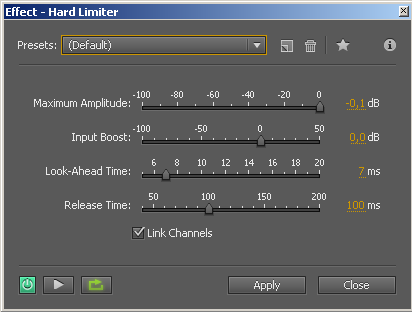
\includegraphics[width=0.55\textwidth]{pic-limiterau-01}}
  \end{block}
\end{frame}

\begin{frame}
  Классический однополосный компрессор реализуется эффектом \emph{Single-band Compressor}.

  \begin{block}{Окно инструмента \emph{Single-band Compressor}}
    \centering{ 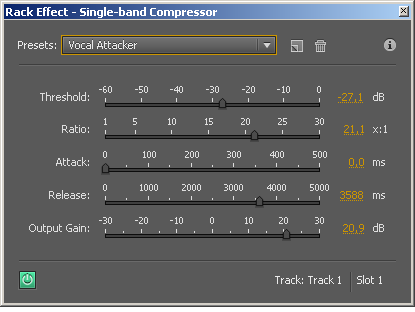
\includegraphics[width=0.65\textwidth]{pic-singleband-01}}
  \end{block}
\end{frame}

\begin{frame}
  Эффект \emph{Amplitude And Compression > Tube-modeled Compressor} имитирует колорит устаревших аппаратных ламповых компрессоров. Использовать данных эффект можно для того, чтобы добавить (едва заметное) искажение типа \emph{distortion}, которое придаст звуку "<приятную окраску">.

  \begin{block}{Окно инструмента \emph{Single-band Compressor}}
    \centering{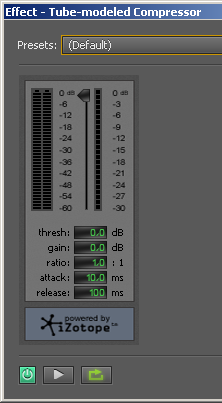
\includegraphics[width=0.25\textwidth]{pic-tubemode-01}}
  \end{block}
\end{frame}

\begin{frame}
  Эффект \emph{Amplitude and Compression > Multiband Compressor} позволяет производить независимую компрессию в четырех различных частотных диапазонах. Так как динамика звука для каждого частотного диапазонах уникальна, то данный эффект является мощным средством для сведения звука.

  \begin{block}{Окно инструмента \emph{Multiband Compressor}}
    \centering{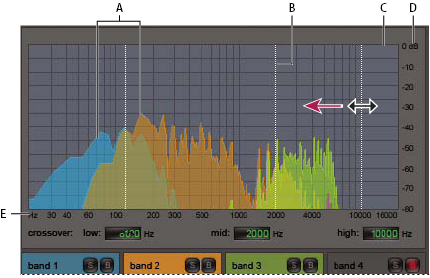
\includegraphics[width=0.55\textwidth]{pic-multiband-01}}
  \end{block}
\end{frame}

\section[Waves Platinum Native Bundle]{Инструменты динамической обработки Waves Platinum Native Bundle}
\begin{frame}
  \emph{Waves RComp}~--- компрессор/экспандер, в котором имитируется устройство с традиционным составом элементов управления.
  
  \begin{block}{Окно инструмента \emph{RComp}}
    \centering{ 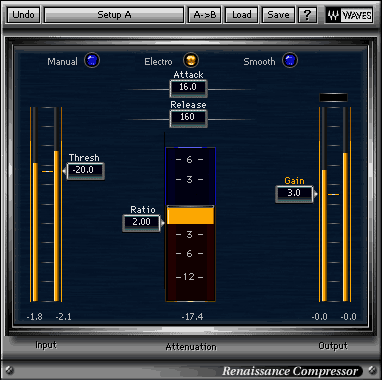
\includegraphics[width=0.55\textwidth]{pic-wavescomp-01}}
  \end{block}
\end{frame}

\begin{frame}
\textbf{Диэсер} представляет собой компрессор, реагирующий на уровень не всего обрабатываемого сигнала, а на уровень его определенных спектральных составляющих. Диэсер получается, когда в канал управления компрессором встраивают фильтр, выделяющий частоты, характерные для свистящих звуков. 

  \begin{block}{Окно инструмента \emph{RDeEsser}}
    \centering{ 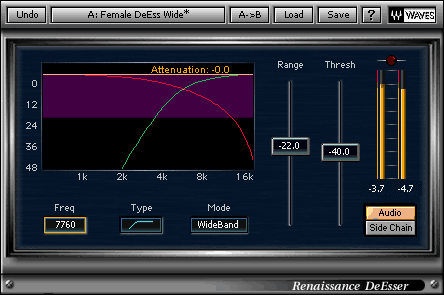
\includegraphics[width=0.65\textwidth]{pic-wavescomp-02}}
  \end{block}
\end{frame}

\begin{frame}
\emph{C1 comp}~--- один из модулей, составляющих линейку виртуальных приборов динамической обработки. В некоторые более сложные приборы \emph{C1 comp} входит в качестве составной части.

  \begin{block}{Окно инструмента \emph{C1 Comp}}
    \centering{ 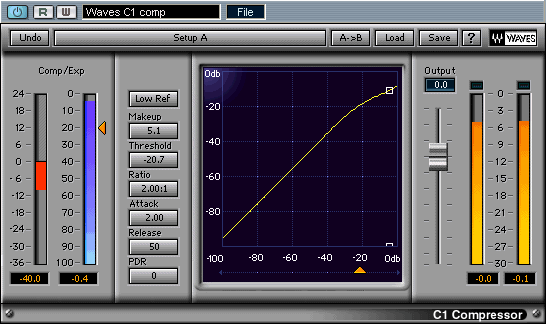
\includegraphics[width=0.75\textwidth]{pic-wavescomp-03}}
  \end{block}
\end{frame}  

\begin{frame}
\emph{C1 gate} представляет собой виртуальный прибор динамической обработки, который в зависимости от состояния элементов настройки может выполнять либо функции гейта, либо функции экспандера.

  \begin{block}{Окно инструмента \emph{C1 gate}}
    \centering{ 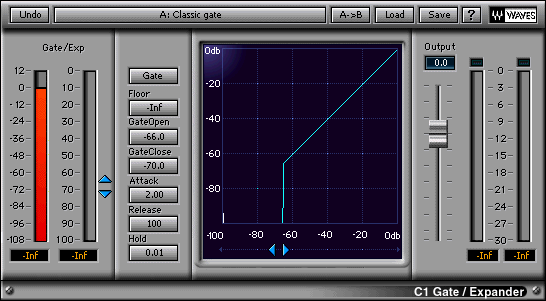
\includegraphics[width=0.75\textwidth]{pic-wavescomp-04}}
  \end{block}
\end{frame} 

\begin{frame}
  \emph{RVox} представляет собой гейт, вокальный компрессор и ограничитель, объединенные в одном плагине, управление которым предельно упрощено за счет того, что предусмотрена автоматическая регулировка уровня входного сигнала, а динамические параметры (времена атаки и освобождения) для изменения недоступны.

  \begin{block}{Окно инструмента \emph{RVox}}
    \centering{ 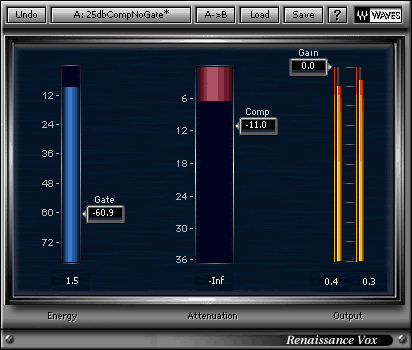
\includegraphics[width=0.5\textwidth]{pic-wavescomp-05}}
  \end{block}
\end{frame} 

\begin{frame}
  Термин "<\emph{Side Chain}"> переводится как "<боковая цепь">. В данном случае имеется в виду канал управления компрессором, в который могут быть включены дополнительные элементы обработки управляющего сигнала.

  ~

  Примером полезного применения боковой цепи может служить диэсер, который получается, если в канал управления компрессором включить фильтр, выделяющий частоты, характерные для свистящих звуков. 
  
  ~
  
  Еще один пример: на вход основного канала компрессора можно подать фоновую музыку, а в канал управления подать сигнал, содержащий речь диктора. Речь без обработки и музыку, обработанную таким компрессором, затем следует смикшировать. В итоге получится, что в паузах музыка будет звучать с нормальной громкостью, а во время разговора будет автоматически приглушаться.
\end{frame}

\begin{frame}
  \begin{block}{Окно инструмента \emph{С1 comp/sidechain}}
    \centering{ 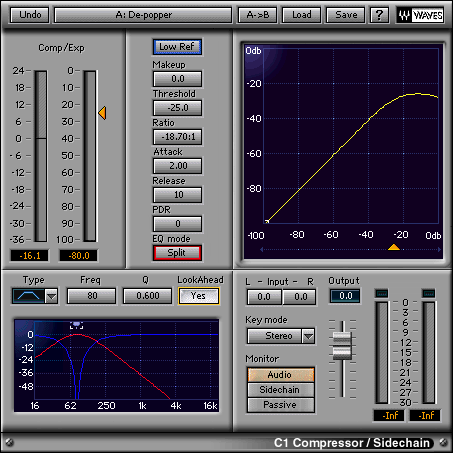
\includegraphics[width=0.65\textwidth]{pic-wavescomp-06}}
  \end{block}
\end{frame} 

\begin{frame}
\emph{C1 comp-gate}~--- универсальный процессор динамической обработки: компрессор, деэсер, экспандер, гейт, а также сочетание двух приборов, включенных последовательно, и многое другое. 

  \begin{block}{Окно инструмента \emph{С1 comp/gate}}
    \centering{ 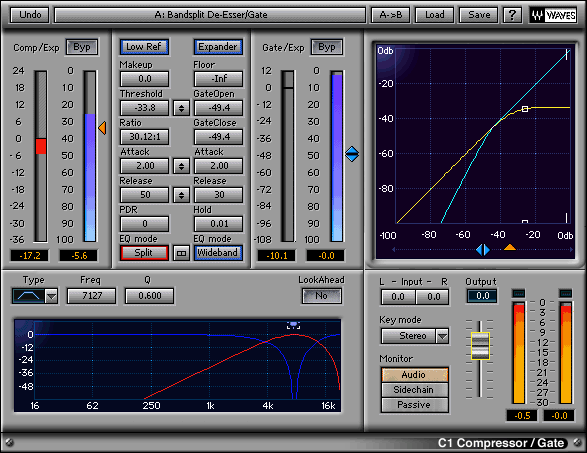
\includegraphics[width=0.65\textwidth]{pic-wavescomp-07}}
  \end{block}
\end{frame} 

\section{Примеры динамической обработки}
\subsection{Пример track01}
\begin{frame}
Часть 1, является качественно записанным на петличный микрофон треком, взятым из документального фильма. Мужская речь имеет неровную динамику, которая могла бы сделать ее трудной для сведения с музыкой или вызвать проблемы в средствах передачи звука с ограниченным диапазоном, таких как телевидение или передача звука по Интернету.

~

В части 2 трека показан результат умеренной компрессии:
\begin{itemize}
  \item степень сжатия 4:1, порог -15~дБ;
  \item время атаки 1~мсек, время восстановления 300~мсек.
\end{itemize}

~

В исходном сигнале имеется довольно низкий фоновый шум, но компрессия делает фон сравнительно более громким.

\end{frame}
\begin{frame}
В части 3 трека используется экспандирование для уменьшения фонового шума. Порог выбран так, чтобы быть ниже самых тихих слов говорящего -40~дБ. Атака равна примерно 1,5~мсек, восстановление равно 50~мсек.

~

В части 4 используется компрессия, сопровождаемая экспандированием (комбинирование обработок для части 2 и части 3). Эта версия придает нашему объекту сильное звучание, делает место съемки чище, и будет более легкой для сведения. Но различия являются тонкими. После ее прослушивания вернитесь к части 1 для сравнения.
\end{frame}

\subsection{Пример track02}
\begin{frame}
Часть 1, является плохо записанным треком документального фильма. При съемке использовался микрофон камеры (почти всегда эта идея является неудачной). Так как объект далеко от микрофона, шум становится громче относительно голоса. Сравнимые расстояния от микрофона до объекта и микрофона до отражающих поверхностей акцентируют эхо помещения.

~

На первом шаге очистки звука следовало бы использовать эквалайзер для создания провала на резонансных частотах помещения и вырезки шума, а также возвращения некоторой энергии в нижние частоты голоса.
\end{frame}

\begin{frame}
В части 2 показано, как гейт может уменьшить очевидный шум. Порог должен быть ниже самых тихих слов; в этом случае он равен -40~dBFS. Так как гейт работает в широком динамическом диапазоне, то есть  вероятность, что фоновые шумы будут щелкать при быстром включении или выключении.

~

Внимательно послушайте часть 2. Проблемы помещения понизились в паузах, но все еще остались во время речи объекта. Если бы трек имел умеренное эхо, то этот способ сделал эхо менее назойливым. Если бы эхо было большим, то оно по-прежнему мешало бы разборчивости речи, даже если бы вы полностью отсекли эхо в паузах.
\end{frame}

\subsection{Пример track03}
\begin{frame}
Часть 1, является комментарием к документальному материалу в стиле программы новостей. Хотя диктор выдерживает довольно постоянный уровень, она стремится подчеркивать слова, повышая как громкость, так и тон.

~

В части 2 исправлено стремление к такому подчеркиванию с помощью компрессора. Порог -12~dBFS, степень сжатия 6:1, атака равна миллисекунде, а восстановление 10мсек. Компенсирующее усиление 4dB.

\end{frame}
\begin{frame}
В части 3 показана предельная степень компрессии. Она разрушает большинство динамики голоса, однако, это может быть полезно при создании спецэффектов или для повышения разборчивости. Степень сжатия 10:1, порог установлен на -20 dB. Атака равна 2 мсек, восстановление - 35мсек. Компенсирующее усиление 10dB.

~

В части 4 показано воздействие на голос де-эссера. Частоты среза: 4 кГц и 12кГц. Нижние частоты оставлены без изменения, поэтому в голосе не ощущается компрессии. Высокие частоты были обработаны со степенью сжатия 8:1 и с подавлением шипящих звуков, примерно равным -6~дБ. В данном случае, порог был установлен -35~дБ. Атака равна 1мсек, восстановление 5мсек; так обработки коснулись только с высокие частоты, то не было необходимости беспокоится об искажениях из-за слишком малого времени реакции.
\end{frame}

\subsection{Пример track04}
\begin{frame}
Компрессоры, экспандеры и гейты полезны для изменения природы звуковых эффектов, как для достижения высокой реалистичности, так и для создания нереальных, неестественных звуков. Пример демонстрирует применение динамической обработки на примере при записи мортиры.

~

Часть 1 является оригинальной записью. Мы стоим довольно близко от мортиры и затем слышим далекое эхо.

~

Часть 2 является результатом компрессии. Хотя звук выстрела остался прежним, он кажется более продолжительным потому, что увеличена первоначальная реверберация. Отдаленное эхо усилено до такой степени, что его звук похож на взрыв снаряда при поражении цели. Сначала эхо было усилено на 10~дБ, а затем к эхо была применена компрессия: степень сжатия 15:1, порог -30~dBFS. Атака равна 3 мсек; восстановление равно 35~мсек. Усиление 18~дБ.

\end{frame}
\begin{frame}
Часть 3 является звуком мортиры, экспандированным ниже порога для того, чтобы оставить только звука выстрела. Без эха это больше похоже на барабан, а не на орудие. Верхний порог -20~dBFS, нижний -40~dBFS. Атака 0.001~мсек, восстановление 50~мсек. Степень сжатия 1:4.
\end{frame}

\subsection{Пример track05}
\begin{frame}
Тот же принцип можно применить и для фоновых звуков. Пример является внутренней атмосферой вагона поезда. Применив небольшую динамическую обработку, вы можете изменить ее характер для более легкого сведения.

Часть 1 является оригинальным звуком. В нем отчетливо слышатся механические шумы.

~

В части 2 использован компрессор для сглаживания этих шумов. Они остаются, но теперь не будут отвлекать от речи. Степень сжатия равна 10:1, а порог был -10~dBFS, атака была равна 0.5~мсек, а восстановление~--- 35~мсек. При таких значениях низкие частоты искажались бы, но шумы находятся в среднем диапазоне.

~

В части 3 предпринят другой подход к улучшению пригодности звука для микса. Экспандер с довольно высоким верхним порогом подавляет большинство фона поезда и акцентирует случайные шумы. Верхний порог был равен -10~dBFS, нижний порог был равен -30~dBFS, время атаки и время восстановления оба были равны 10 мсек.
\end{frame}

\subsection{Пример track06}
\begin{frame}
Пример показывает, как динамическая обработка может изменить характер шагов.

~

Часть 1 является мужскими шагами - кожаные ботинки по деревянному полу.

~

В части 2 используется экспандер, чтобы превратить ботинки в туфли на высоких каблуках.

~

Часть 3 является ходьбой в кроссовках по хрустящему бетону.

~

В части 4 взят эффект хрустящего бетона и использован компрессор, чтобы сделать бетон звучащим "<грязнее">.
\end{frame}

\subsection{Пример track07}
\begin{frame}
Пример показывает, как большое время атаки может изменить характер грохота.

~

Часть 1 является звуком оркестровой тарелки, по которой ударили палочкой.

~

Часть 2 является той же записью, только теперь она звучит так, будто по инструменту провели щеткой.
\end{frame}

\end{document}
